\documentclass[a4paper, 12pt]{article}
\usepackage[top=2cm, bottom=2cm, left=2.5cm, right=2.5cm]{geometry}
\usepackage[utf8]{inputenc}
\usepackage[brazilian]{babel}
\usepackage{indentfirst}
\usepackage{graphicx}
\usepackage{wrapfig}
\usepackage[pdftex]{hyperref}
\usepackage{amsmath}
\usepackage{subcaption}

\begin{document}
	\begin{center} %centralizar o texto abaixo
		{\Large Exponencial matricial e simulação com representação de estados}\\[0.4cm]
		{\large Erik Yuji Goto}\\[0.2cm]
		{\normalsize RA: 234009}
	\end{center} %término do comando centralizar

\section{Sistema de Segunda Ordem}
	A equação do movimento escrita na forma padronizada é:	
	\begin{equation}
		\ddot{q} + 2\xi \omega_n \dot{q} + \omega_n^2q = 0
	\end{equation}
	Substituindo pelos valores do enunciado:	
	\begin{equation}
		\ddot{q} + 10\dot{q} + 10^4q = 0
	\end{equation}
	Com isso podemos transformar a equação para a forma matricial:
	\begin{figure}[h]
		\centering
		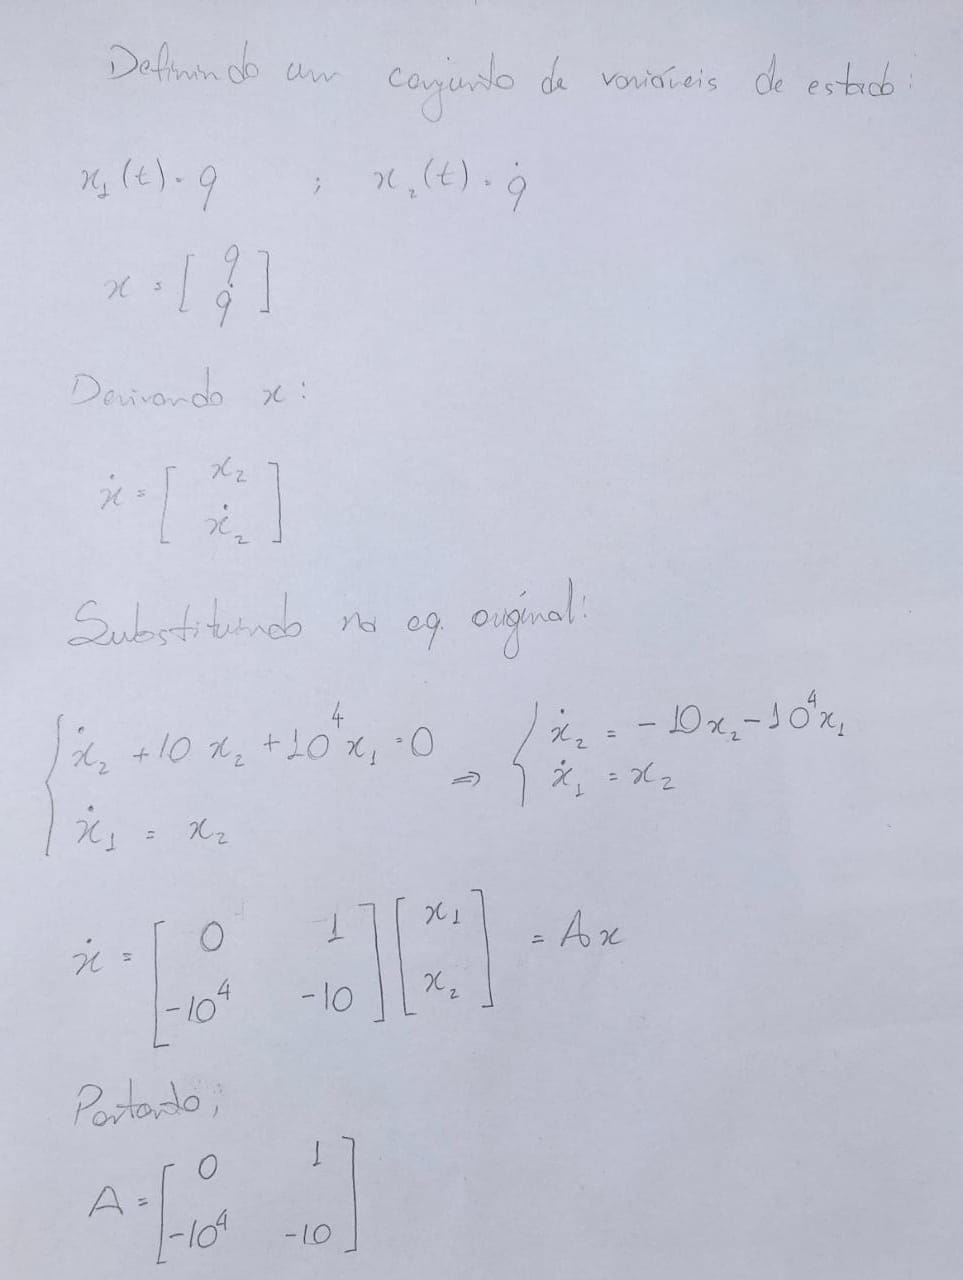
\includegraphics[scale=0.35]{imagens/a1.jpg}
		\caption{Encontrando a matriz A}
	\end{figure}
	\newpage
	Portanto,
	\begin{equation}
		\dot{x} = Ax + Bu
	\end{equation}
	Onde,
	\begin{equation}
		Bu = 0
	\end{equation}
	\begin{equation}
		A = \begin{bmatrix}
		0 & 1\\
		-10^4 & -10
		\end{bmatrix}
	\end{equation}

\section{Calculando a resposta livre}
	A resposta livre a uma condição inicial é dada por:
	\begin{equation}
		x(t) = e^{At} x_0
	\end{equation}
	Portanto, precisamos calcular $e^{At}$
	
	\subsection{Por Autovalores}
		\begin{figure}[h]
			\centering
			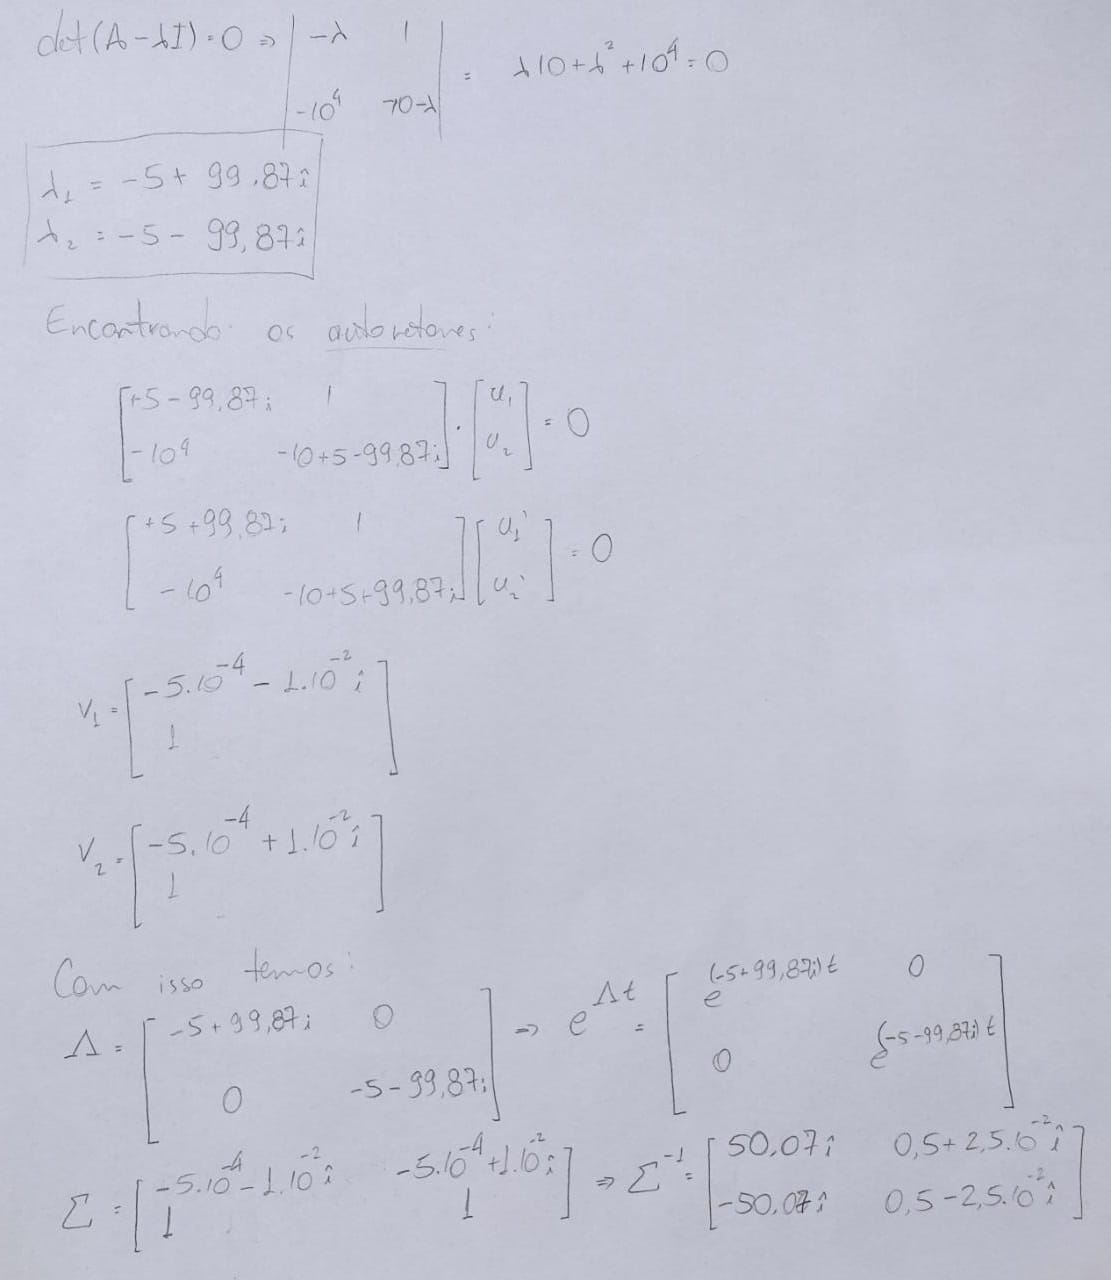
\includegraphics[scale=0.3]{imagens/a2.jpg}
			\caption{Autovalores}
		\end{figure}
		Realizando o cálculo de $e^{At}$ pelo matlab:
		\begin{center}
			$syms \texttt{ t};$\\
			$[U,L] = eig(A);$\\
			$e^{At} = U*diag(exp(diag(L*t)))*inv(U)$\\
		\end{center}				
		
		\begin{equation}
			e^{At} = \begin{bmatrix}
				a & b\\
				c & d
			\end{bmatrix}
		\end{equation}
		Onde,\\
		
		$a = (exp(-t*(5 + 399^(1/2)*5i))*(exp(399^(1/2)*t*10i)*(649037107316853271723688571817328 - 32492496402889698541231938784245i) + 649037107316853363837439069708896\\ + 32492496402889703152687390203090i))/1298074214633706907132624082305024$\\
		
		$b = - exp(t*(- 5 + 399^(1/2)*5i))*(10001^(1/2)/200 + 3607572128482979i/144115188075855872)*(4611455451418845/9223372036854775808 + 5757109406118223i/576460752303423488) - exp(-t*(5 + 399^(1/2)*5i))*(10001^(1/2)/200 - 7215144256965959i/288230376151711744)*(4611455451418845/9223372036854775808 - 5757109406118223i/576460752303423488)$\\
		
		$c = (25*10001^(1/2)*exp(-t*(5 + 399^(1/2)*5i))*(exp(399^(1/2)*t*10i)*7046039313443321i - 7046039313443322i))/351878905260408832$\\
		
		$d = (100*10001^(1/2)*exp(t*(- 5 + 399^(1/2)*5i))*(10001^(1/2)/200 + 3607572128482979i/\\144115188075855872))/10001 + (100*10001^(1/2)*exp(-t*(5 + 399^(1/2)*5i))*(10001^(1/2)/200 - 7215144256965959i/288230376151711744))/10001$\\
		

	\subsection{Por Laplace}
		Usaremos a relação $e^{At} = L^{-1}[(sI-A)^{-1}]$
		\begin{figure}[h]
			\centering
			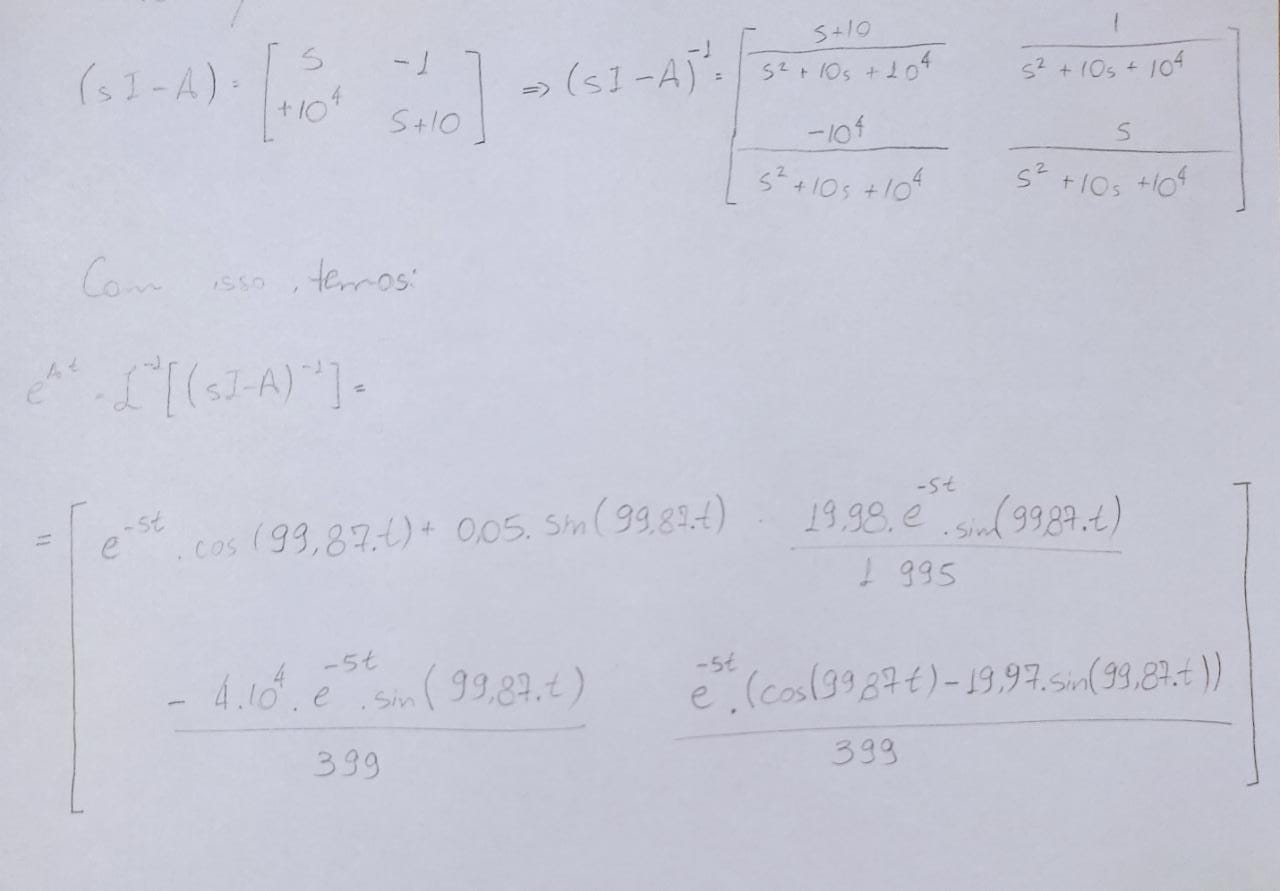
\includegraphics[scale=0.3]{imagens/a3.jpg}
			\caption{Laplace}
		\end{figure}
		
	\subsection{Por Cayley-Hamilton}
		Usamos a equação $e^{At} = \sum^{n-1}_{l = 0} \alpha_lA^l$
		Para encontrar as constantes $\alpha_l$ resolvemos o sistema de equações:
		





	
	
	
	
	
\end{document}